\section{Introducción al radar}
\subsection{Espectro electromagnético}
\begin{frame}{\secname : \subsecname}
  \begin{figure}
    \centering
    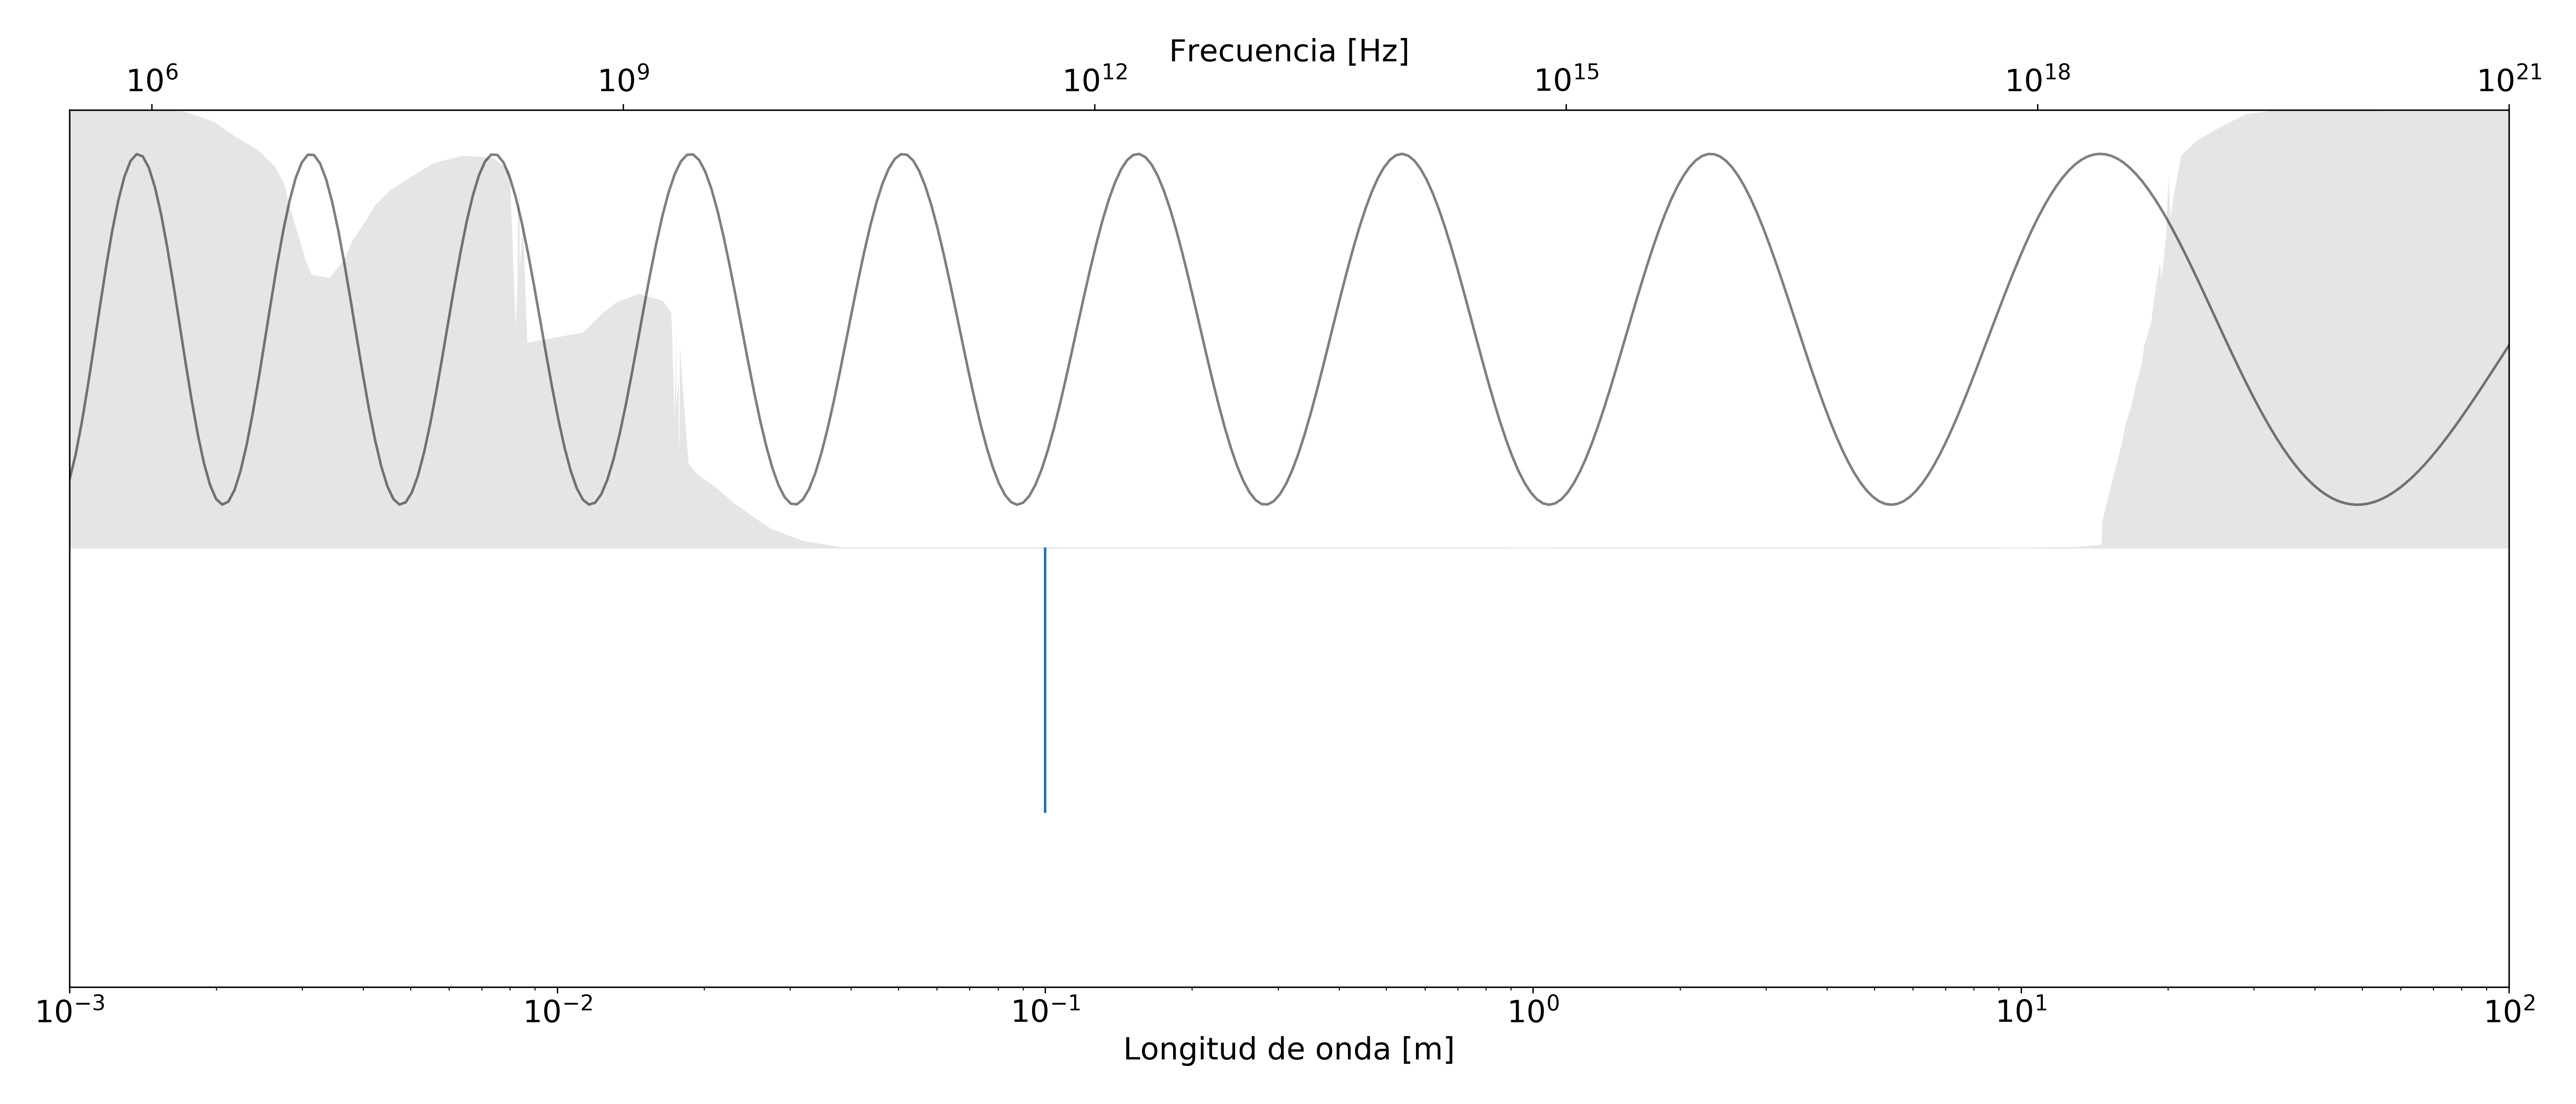
\includegraphics[width=\textwidth]{fig:espectro.png}
    \caption{Espectro electromagnético en longitud de onda (abajo) y frecuencia (arriba).}
    \label{}
  \end{figure}
\end{frame}
%--- Next Frame ---%

\subsection{Funcionamiento de un radar}
\begin{frame}{\secname : \subsecname}
    \begin{figure}
      \centering
      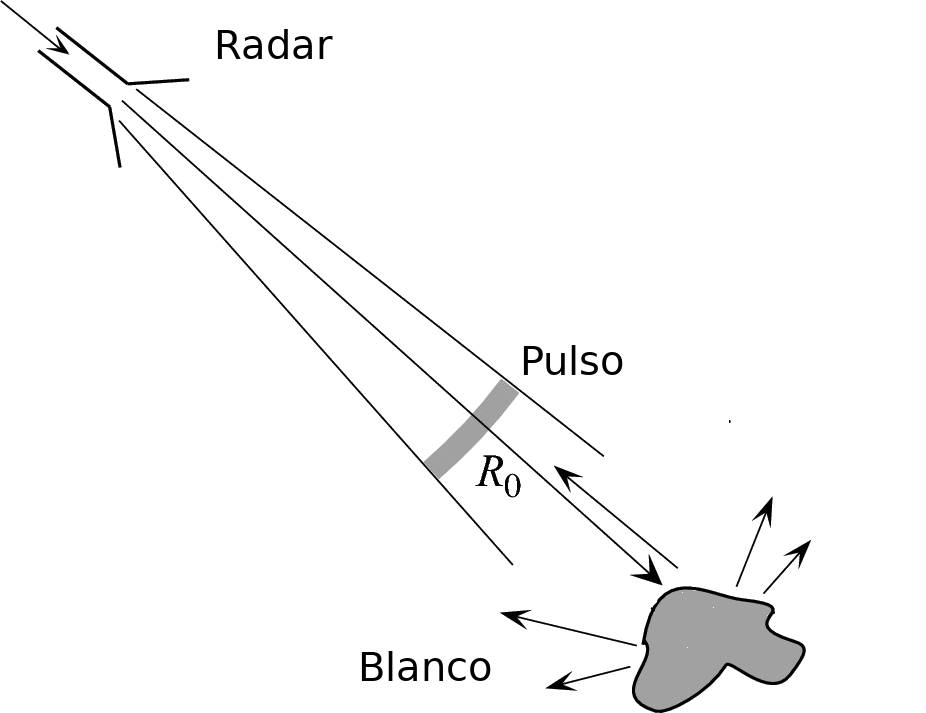
\includegraphics[scale=0.7]{fig:radar.png}
      \caption{RAdio Detection And Ranging. Funcionamiento esquemático.}
      \label{}
    \end{figure}
\end{frame}
%--- Next Frame ---%

\begin{frame}{\secname : \subsecname}
  \begin{figure}
    \centering
    \movie[width = \textwidth,loop,autostart]{\centering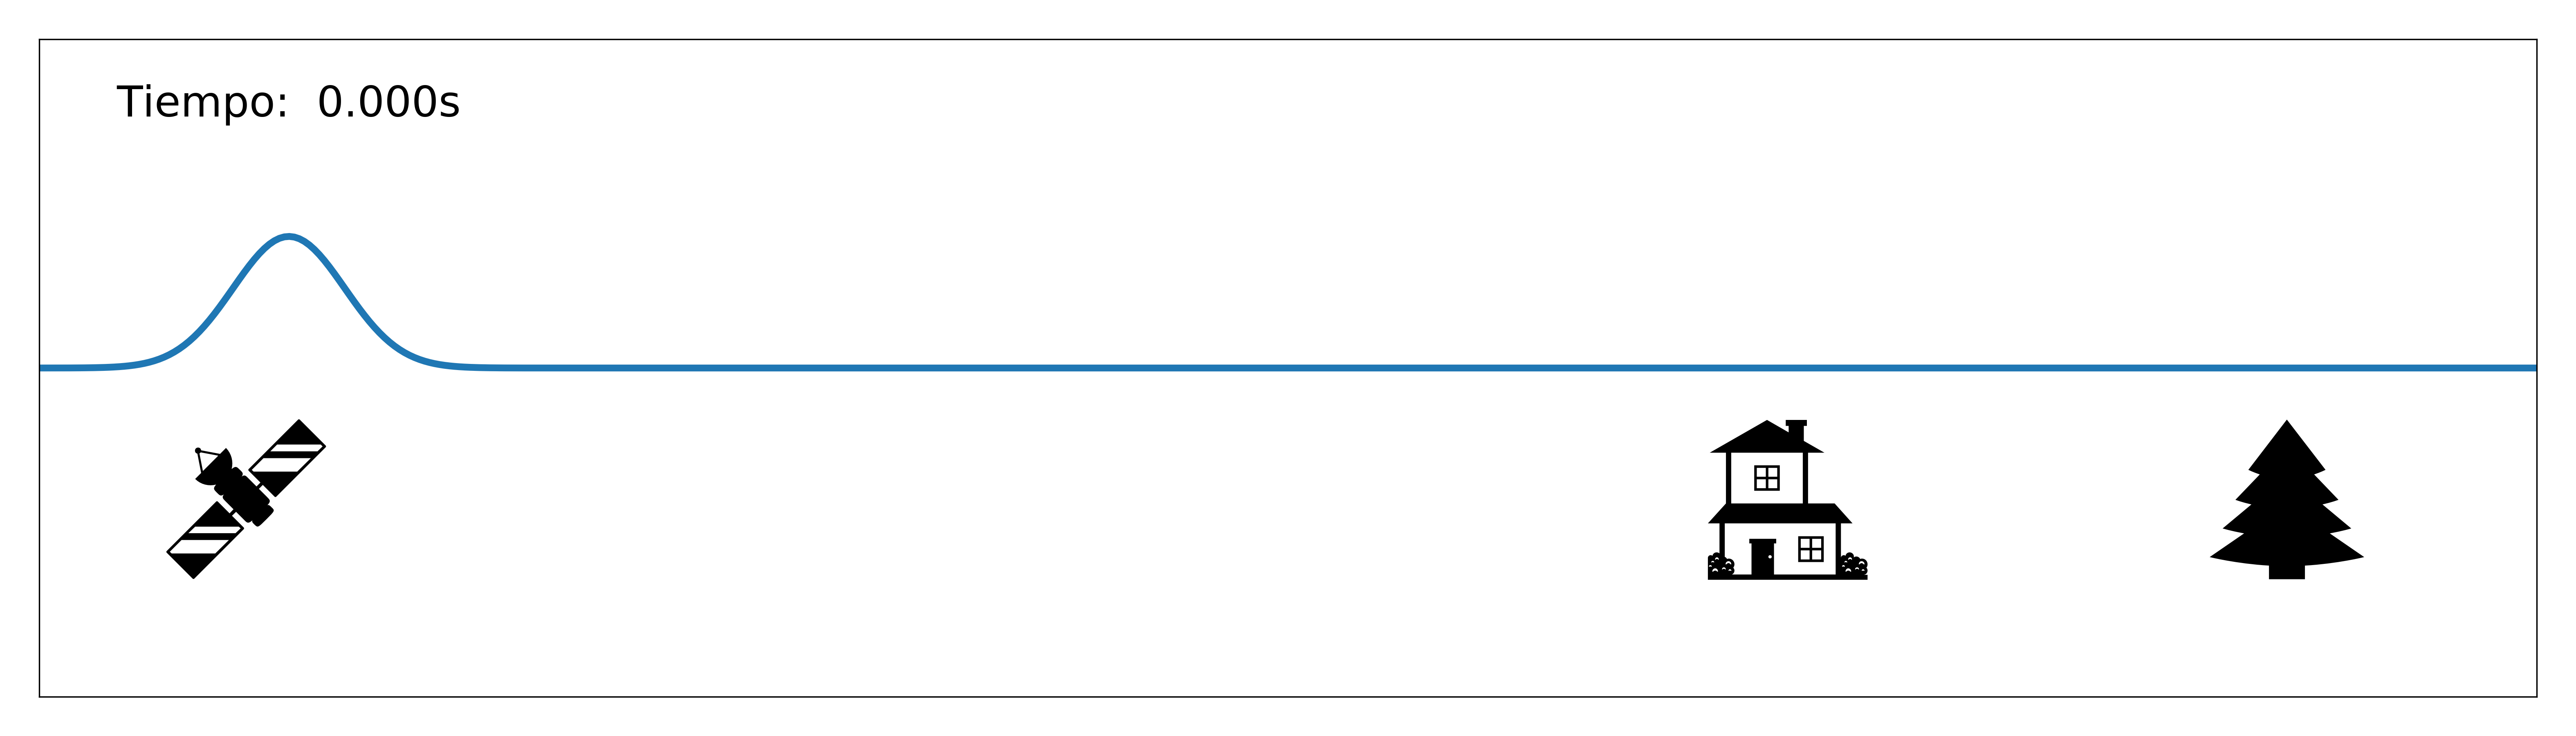
\includegraphics[width=\textwidth]{fig:funcionamiento.png}}{./figs/fig:funcionamiento.mp4}
    \caption{Ecos detectados por un radar en función del tiempo}
    \label{}
  \end{figure}
\end{frame}
%--- Next Frame ---%

\begin{frame}{\secname : \subsecname}
  \begin{figure}
    \centering
    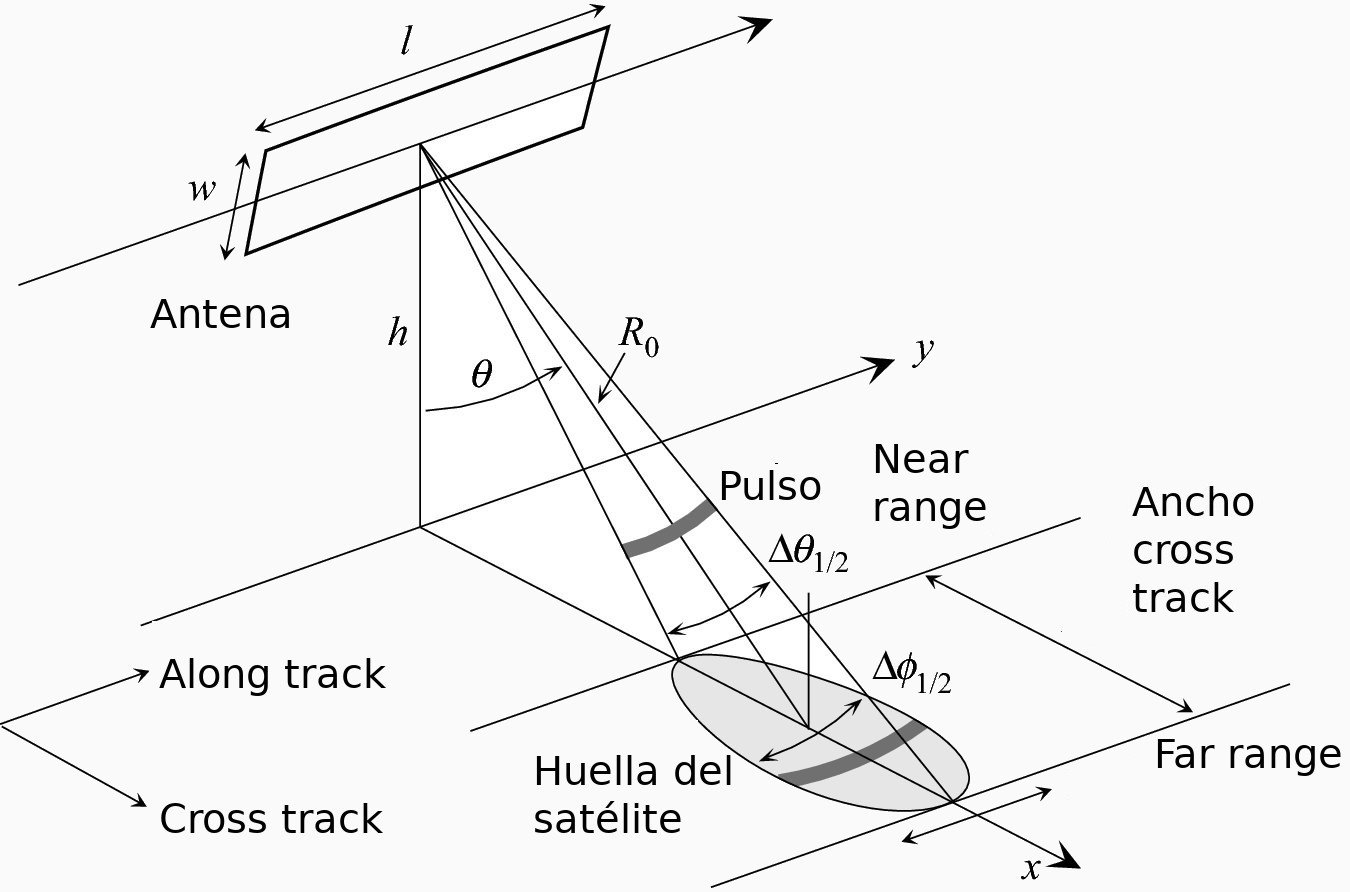
\includegraphics[scale=0.7]{01938fig13_1.jpg}
    \caption{Geometría de observación de un radar completa en la direcciones perpendiculares y paralelas al movimiento (accross track y along track)}
    \label{}
  \end{figure}
\end{frame}
%--- Next Frame ---%


\begin{frame}{\secname : \subsecname}
  \begin{figure}
    \centering
    \movie[width = 0.95\textwidth,loop,autostart]{\centering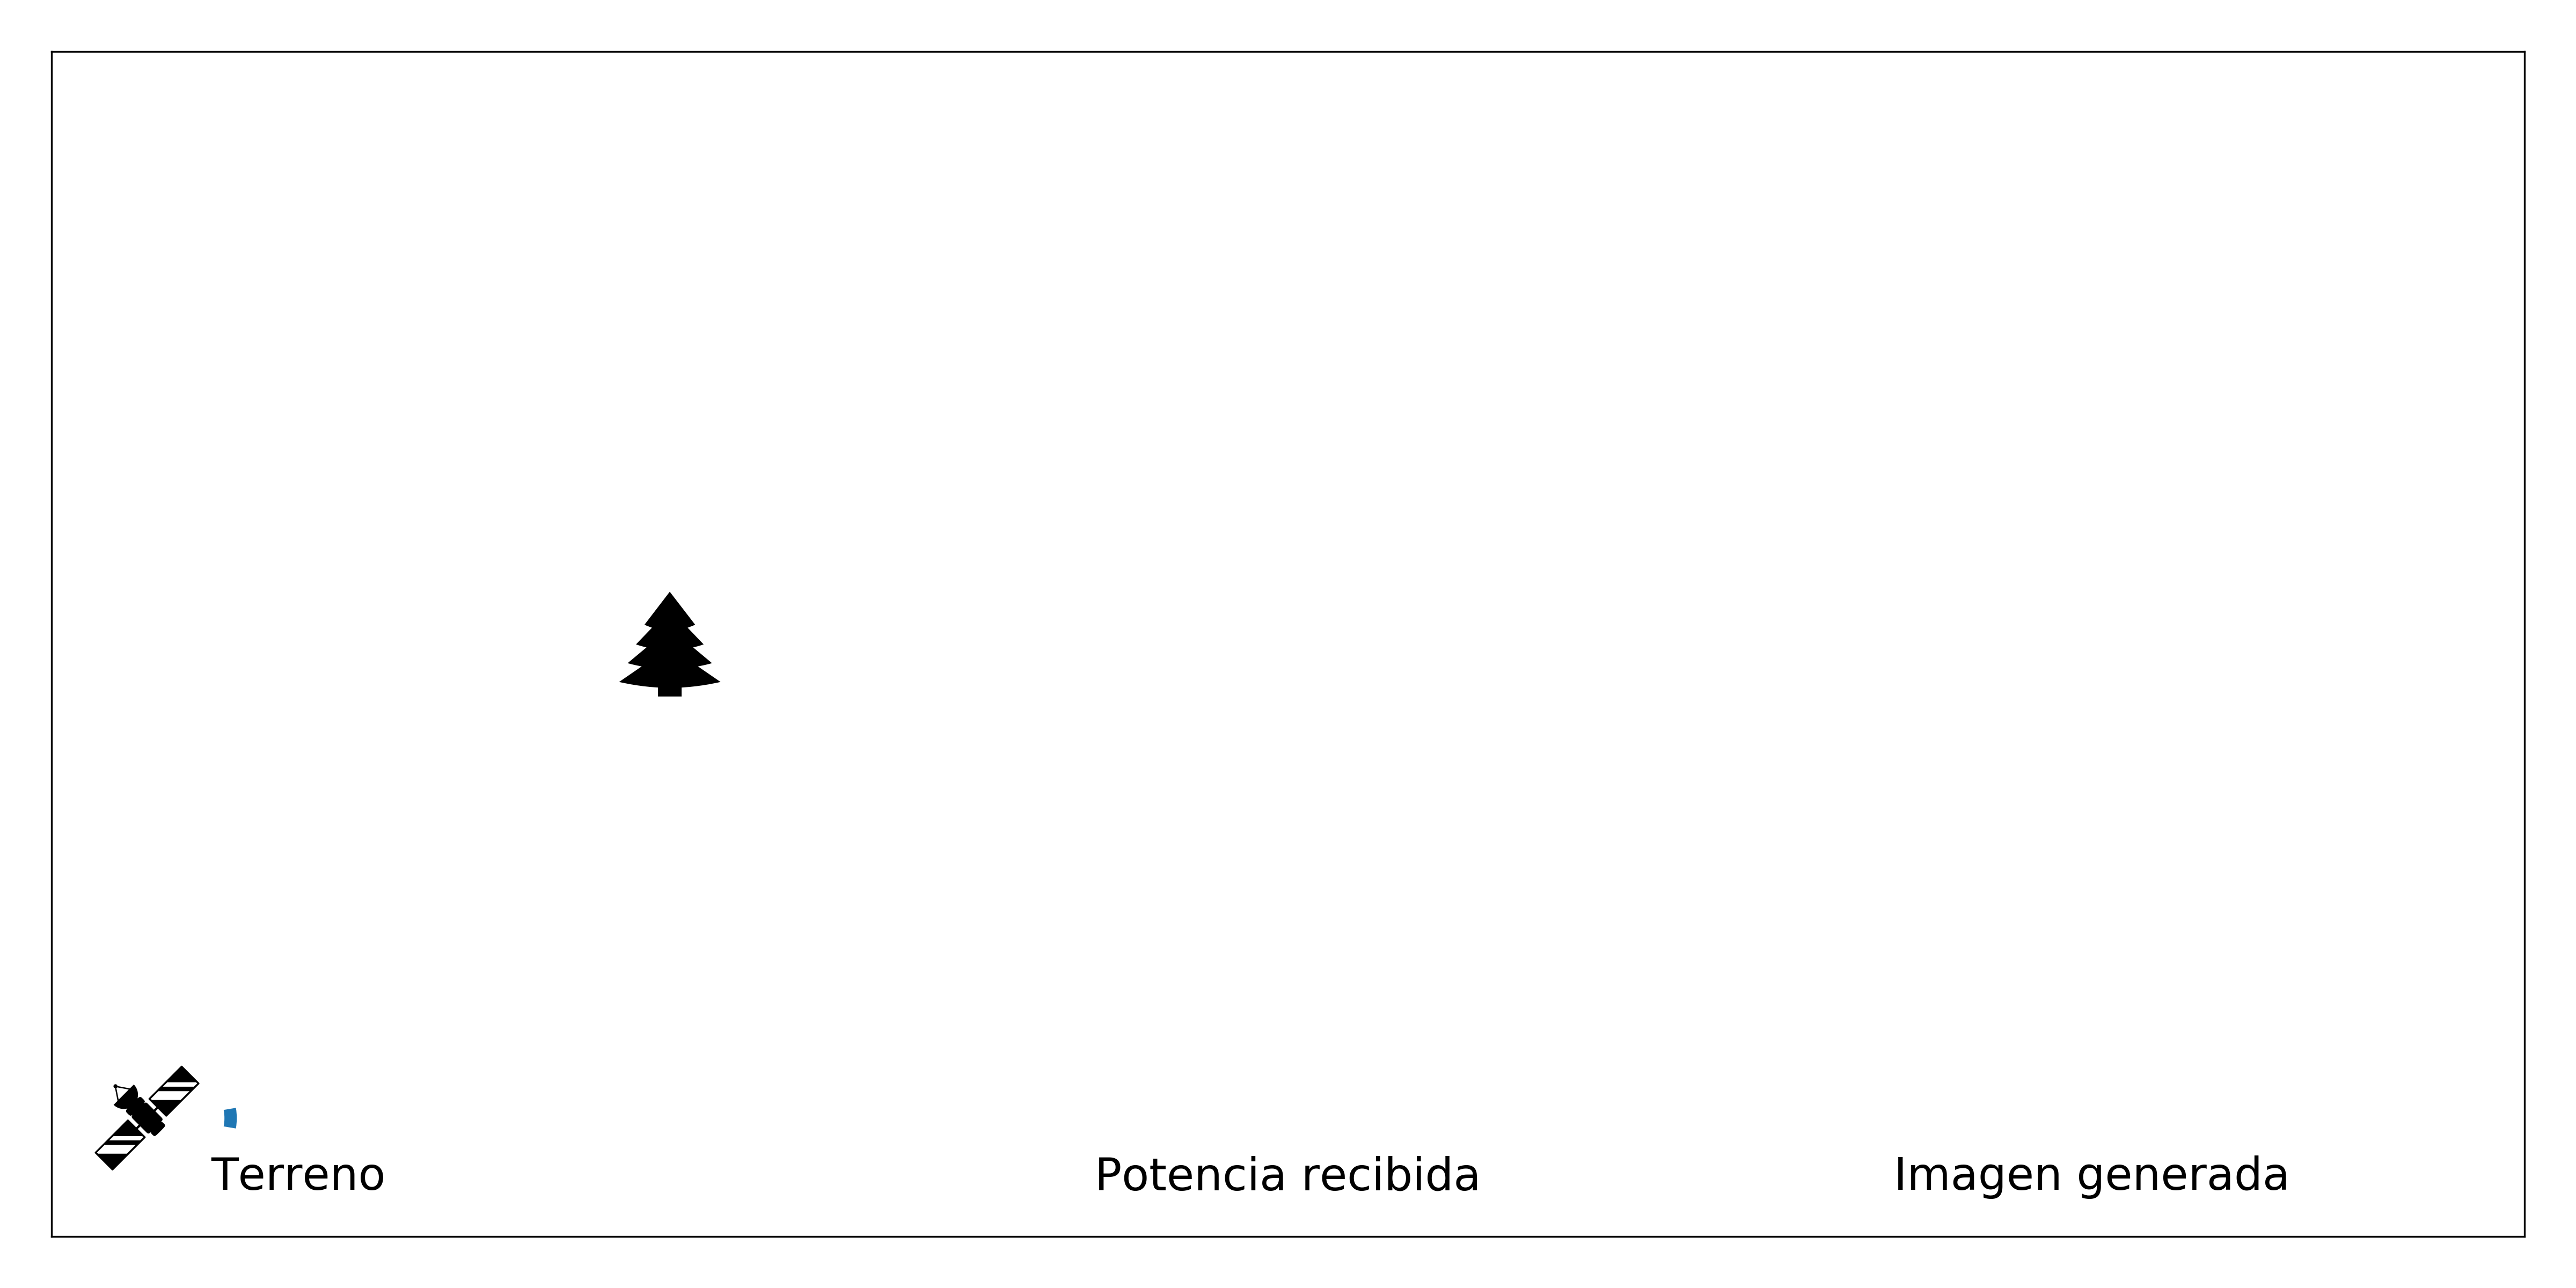
\includegraphics[width=0.95\textwidth]{fig:imagen.png}}{./figs/fig:imagen.mp4}
    \caption{Generación de una imagen radar a partir de datos en el terreno.}
    \label{}
  \end{figure}
\end{frame}
%--- Next Frame ---%

\subsection{Modos de adquisición}

\begin{frame}{\secname : \subsecname}
  \begin{columns}
    \begin{column}{0.5\textwidth}
       \begin{figure}
         \centering
         \movie[width = 0.95\textwidth,loop,autostart]{\centering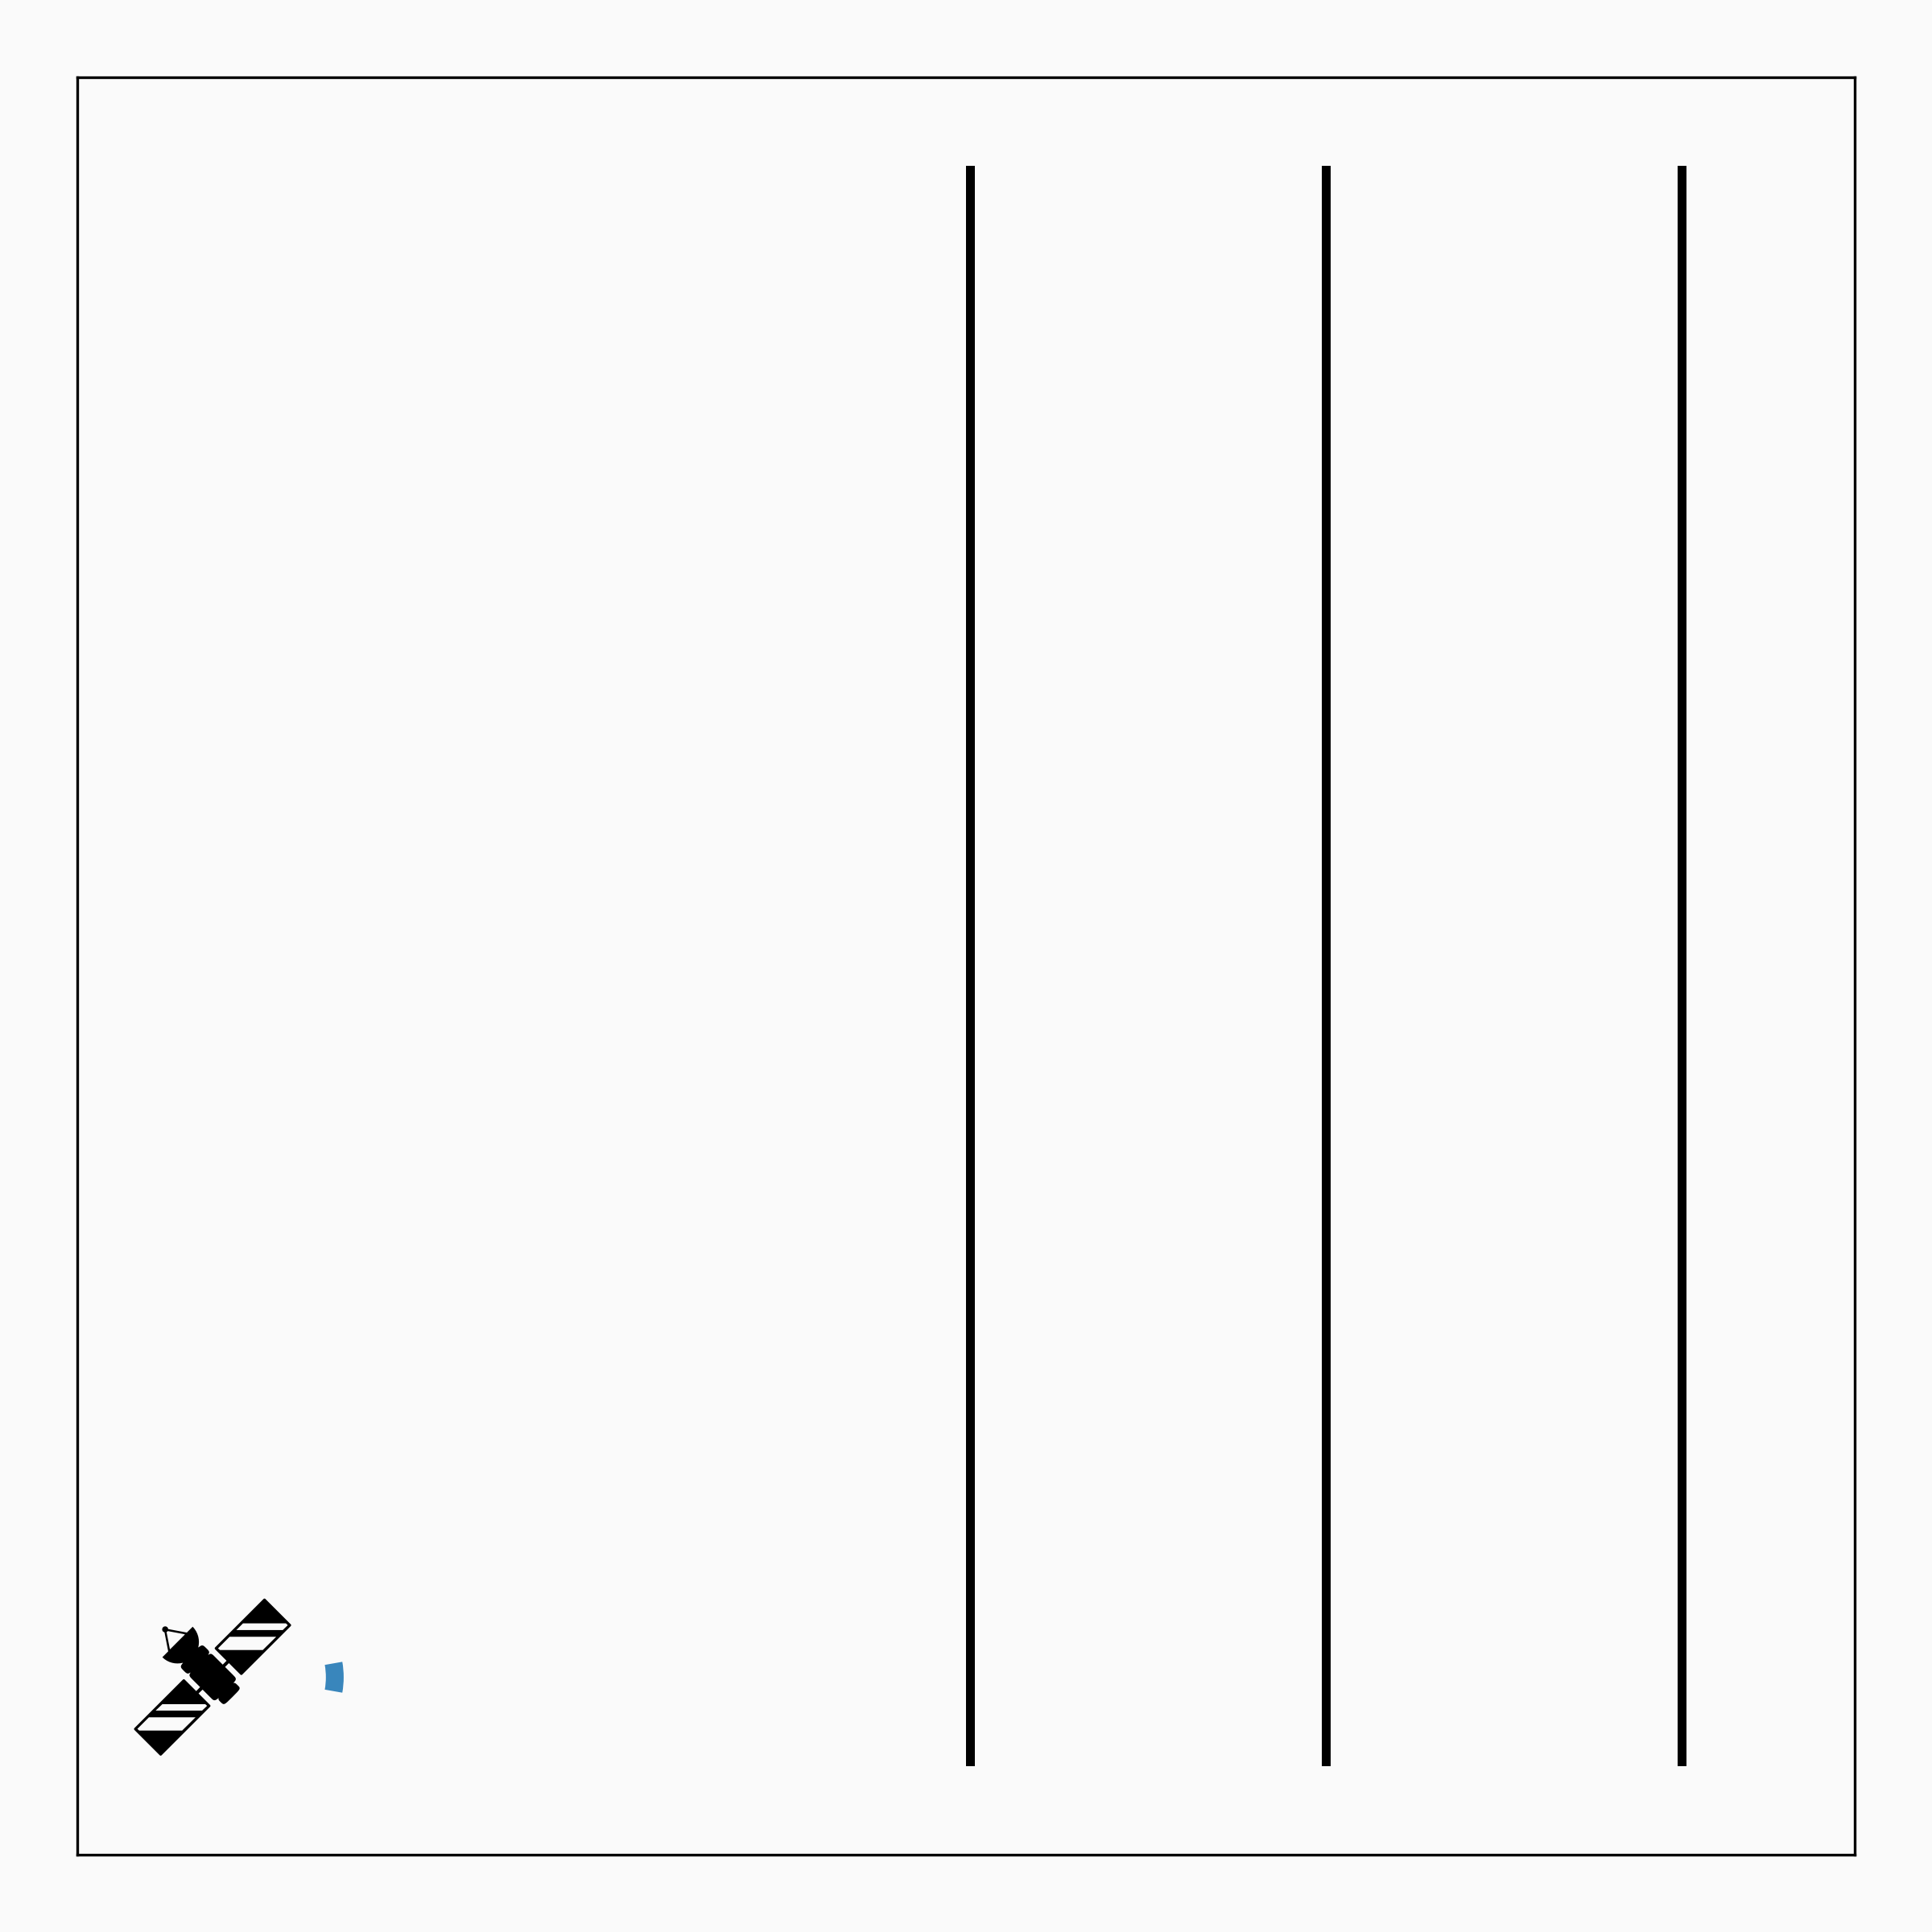
\includegraphics[width=0.95\textwidth]{fig:strip.png}}{./figs/fig:strip.mp4}
         %\caption{Modo de adquisición STRIPMAP.}
         \label{}
       \end{figure}
    \end{column}
    \begin{column}{0.5\textwidth}  %%<--- here
      \begin{block}{Modo de adquisición STRIPMAP}
        \begin{itemize}
          \item El RADAR toma datos de un solo Swadth
          \item Es el método de más básico de adquisición.
          \item Resolución espacial intermedia.
          \item Cobertura limitada.
        \end{itemize}
      \end{block}
    \end{column}
    \end{columns}
\end{frame}
%--- Next Frame ---%

\begin{frame}{\secname : \subsecname}
  \begin{columns}
    \begin{column}{0.5\textwidth}
       \begin{figure}
         \centering
         \movie[width = 0.95\textwidth,loop,autostart]{\centering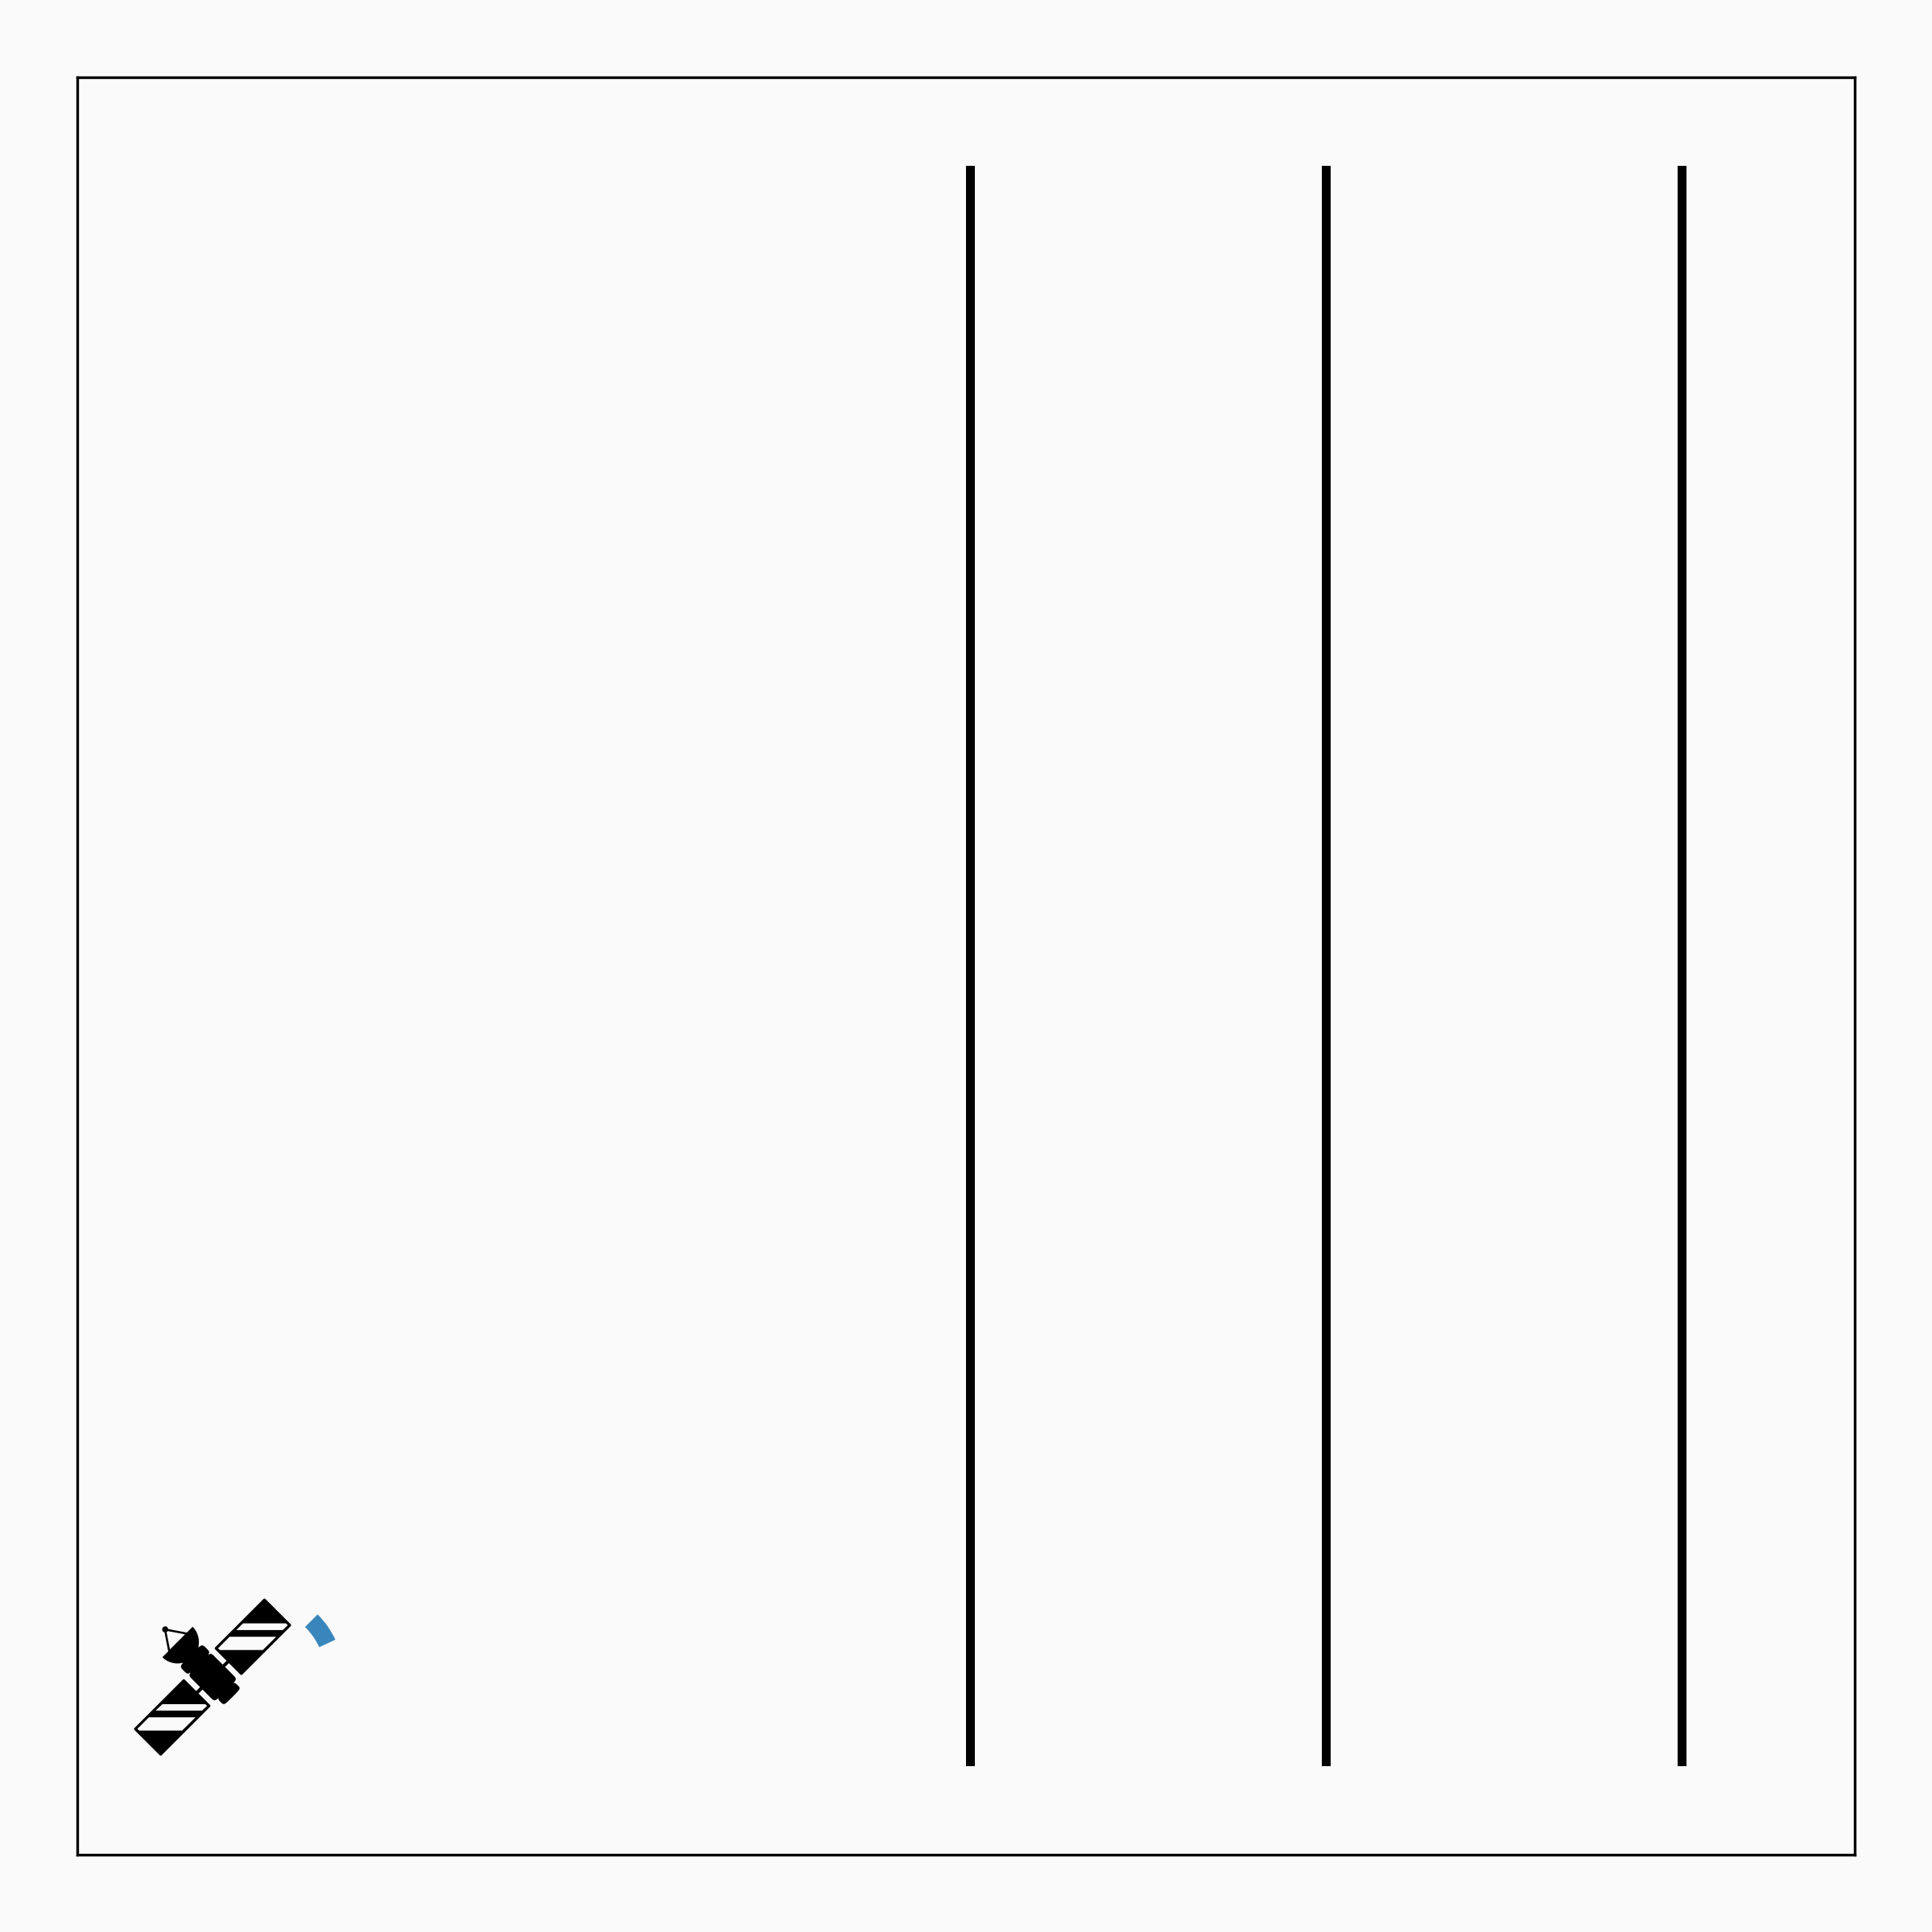
\includegraphics[width=0.95\textwidth]{fig:spot.png}}{./figs/fig:spot.mp4}
         %\caption{Modo de adquisición STRIPMAP.}
         \label{}
       \end{figure}
    \end{column}
    \begin{column}{0.5\textwidth}  %%<--- here
      \begin{block}{Modo de adquisición SPOTLIGHT}
        \begin{itemize}
          \item El RADAR observa un único blanco durante toda la pasada.
          \item Alta resolución espacial.
          \item Baja cobertura.
          \item Necesita reorientar la antena dentro de la adquisición.
        \end{itemize}
      \end{block}
    \end{column}
    \end{columns}
\end{frame}
%--- Next Frame ---%

\begin{frame}{\secname : \subsecname}
  \begin{columns}
    \begin{column}{0.5\textwidth}
       \begin{figure}
         \centering
         \movie[width = 0.95\textwidth,loop,autostart]{\centering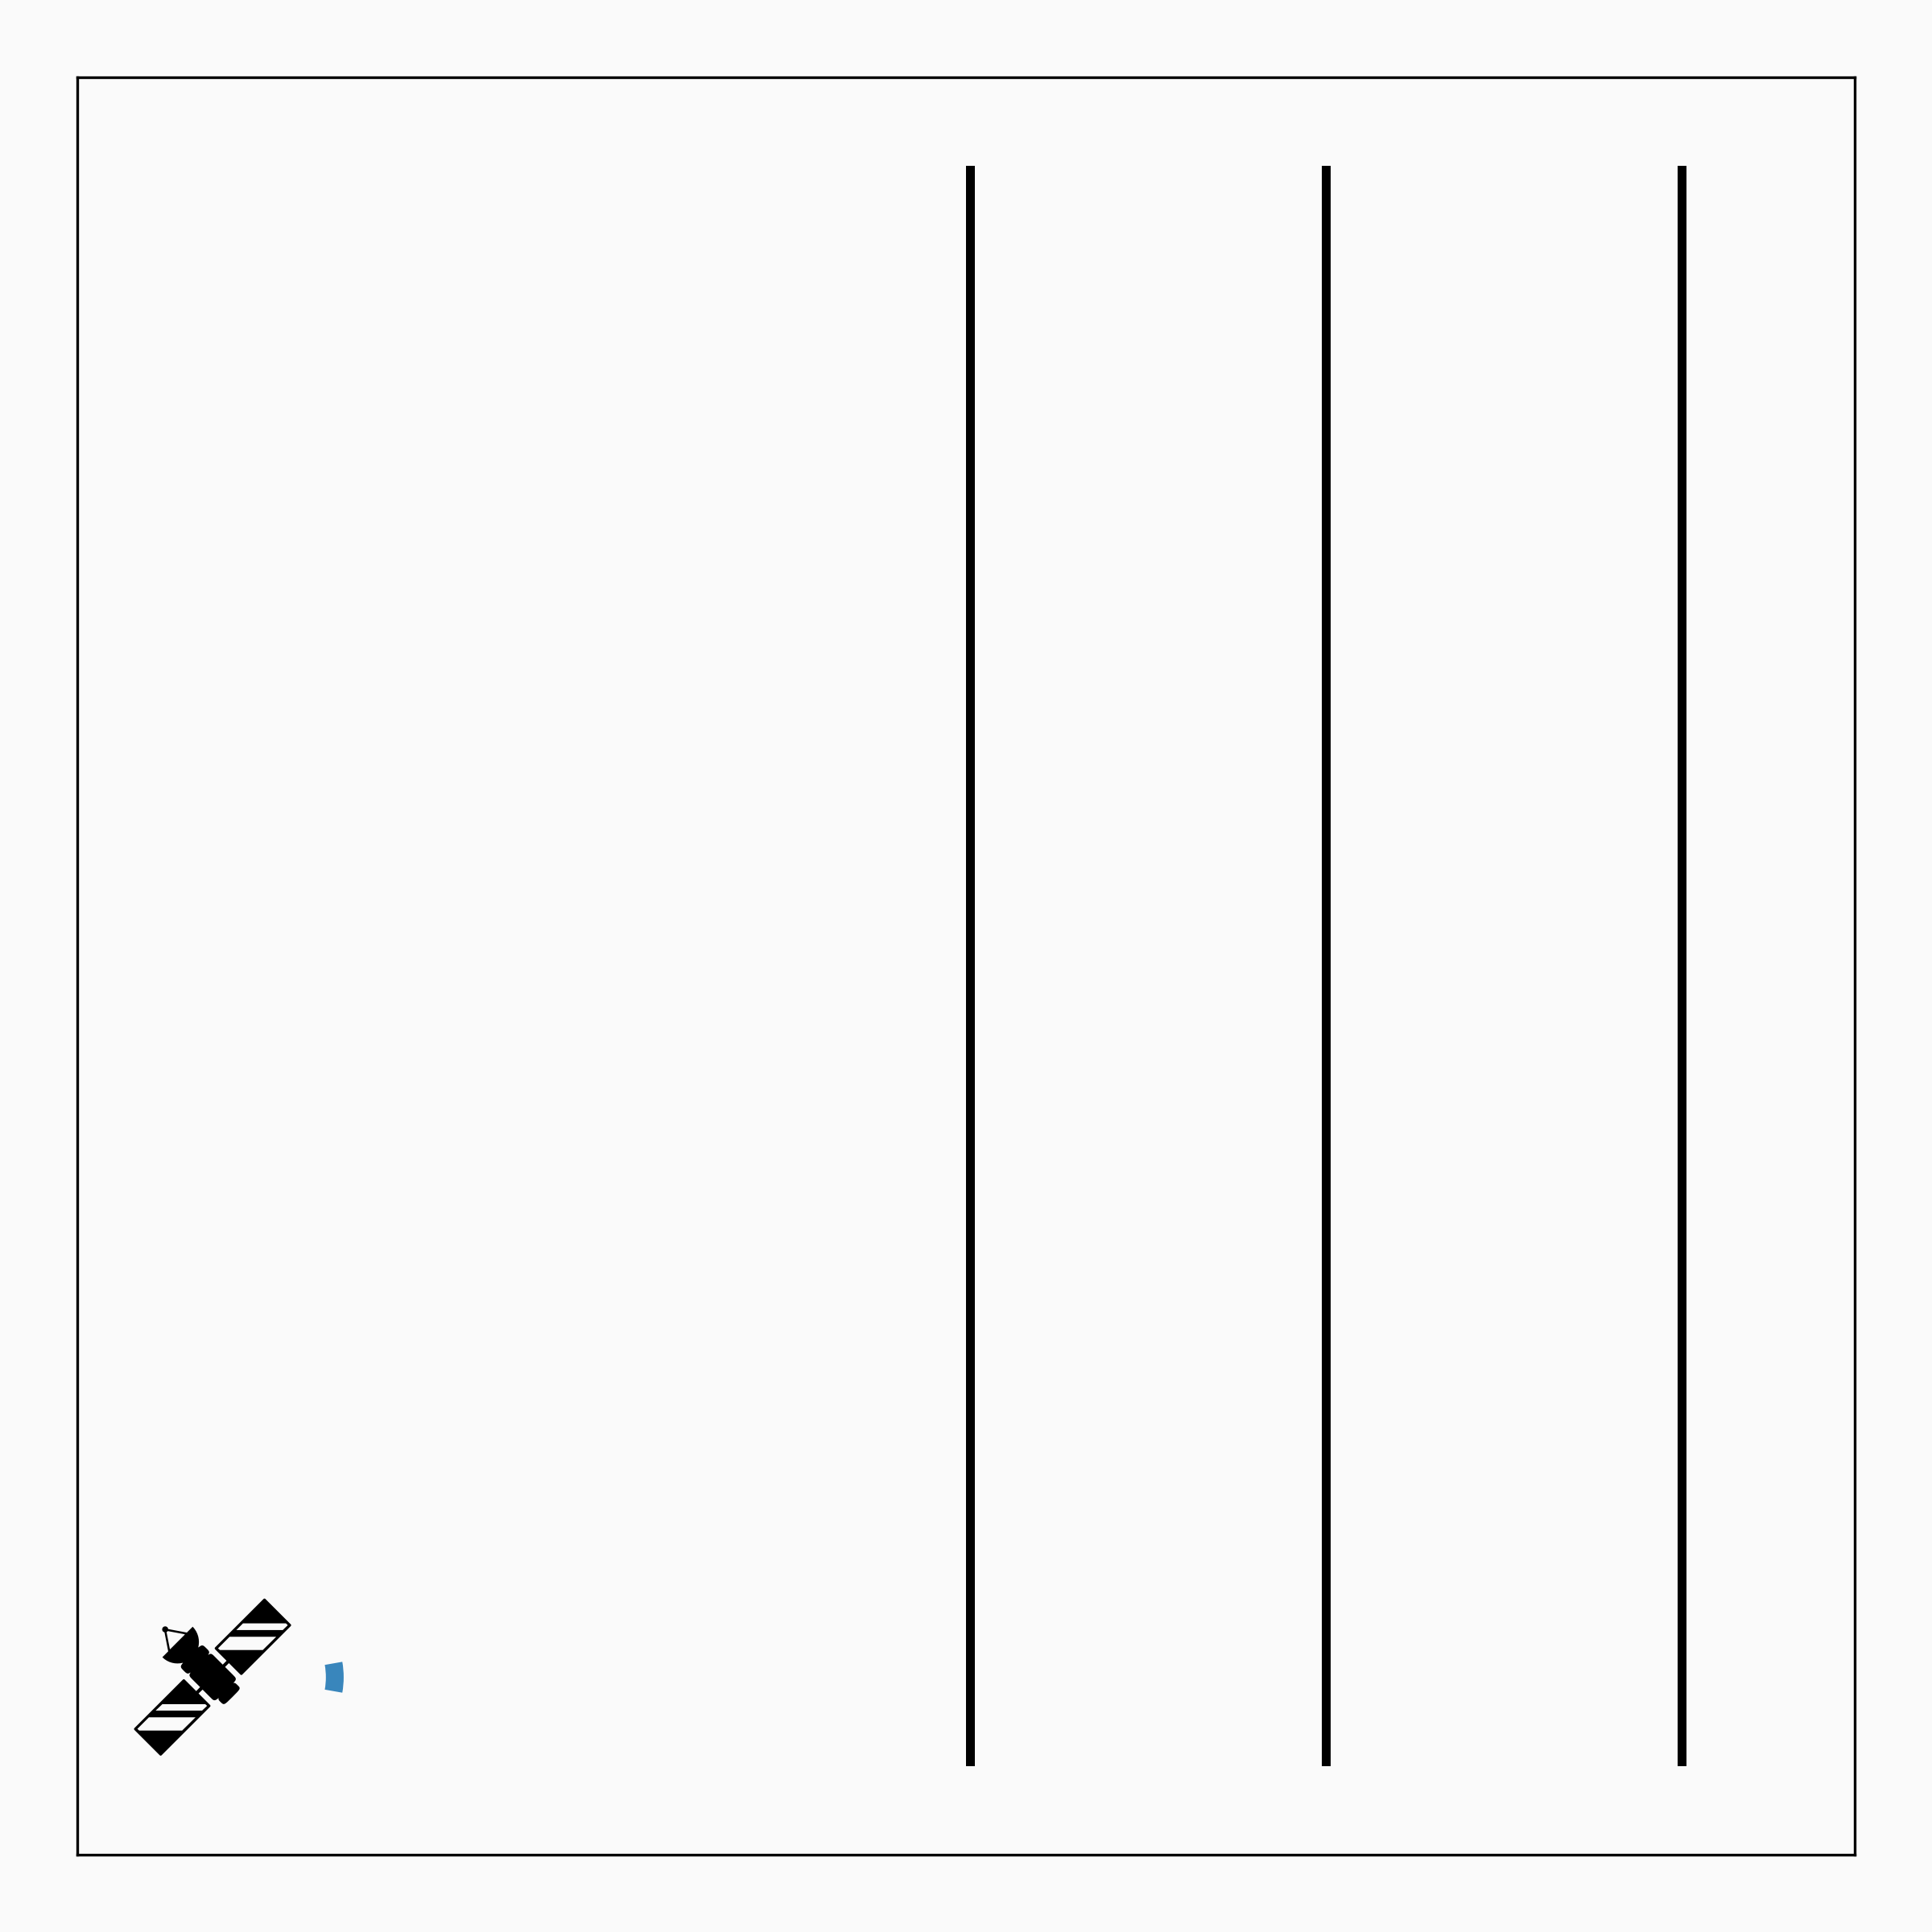
\includegraphics[width=0.95\textwidth]{fig:scan.png}}{./figs/fig:scan.mp4}
         %\caption{Modo de adquisición STRIPMAP.}
         \label{}
       \end{figure}
    \end{column}
    \begin{column}{0.5\textwidth}  %%<--- here
      \begin{block}{Modo de adquisición SCANSAR}
        \begin{itemize}
          \item El RADAR Va distribuyendo pulsos de a bursts entre varios swaths.
          \item Baja resolución.
          \item Gran cobertura.
          \item Mala distribución espacial de potencia.
          \item Hace falta reapuntar la antena en elevación entre burst.
        \end{itemize}
      \end{block}
    \end{column}
    \end{columns}
\end{frame}
%--- Next Frame ---%
\begin{frame}{\secname : \subsecname}
  \begin{columns}
    \begin{column}{0.5\textwidth}
       \begin{figure}
         \centering
         \movie[width = 0.95\textwidth,loop,autostart]{\centering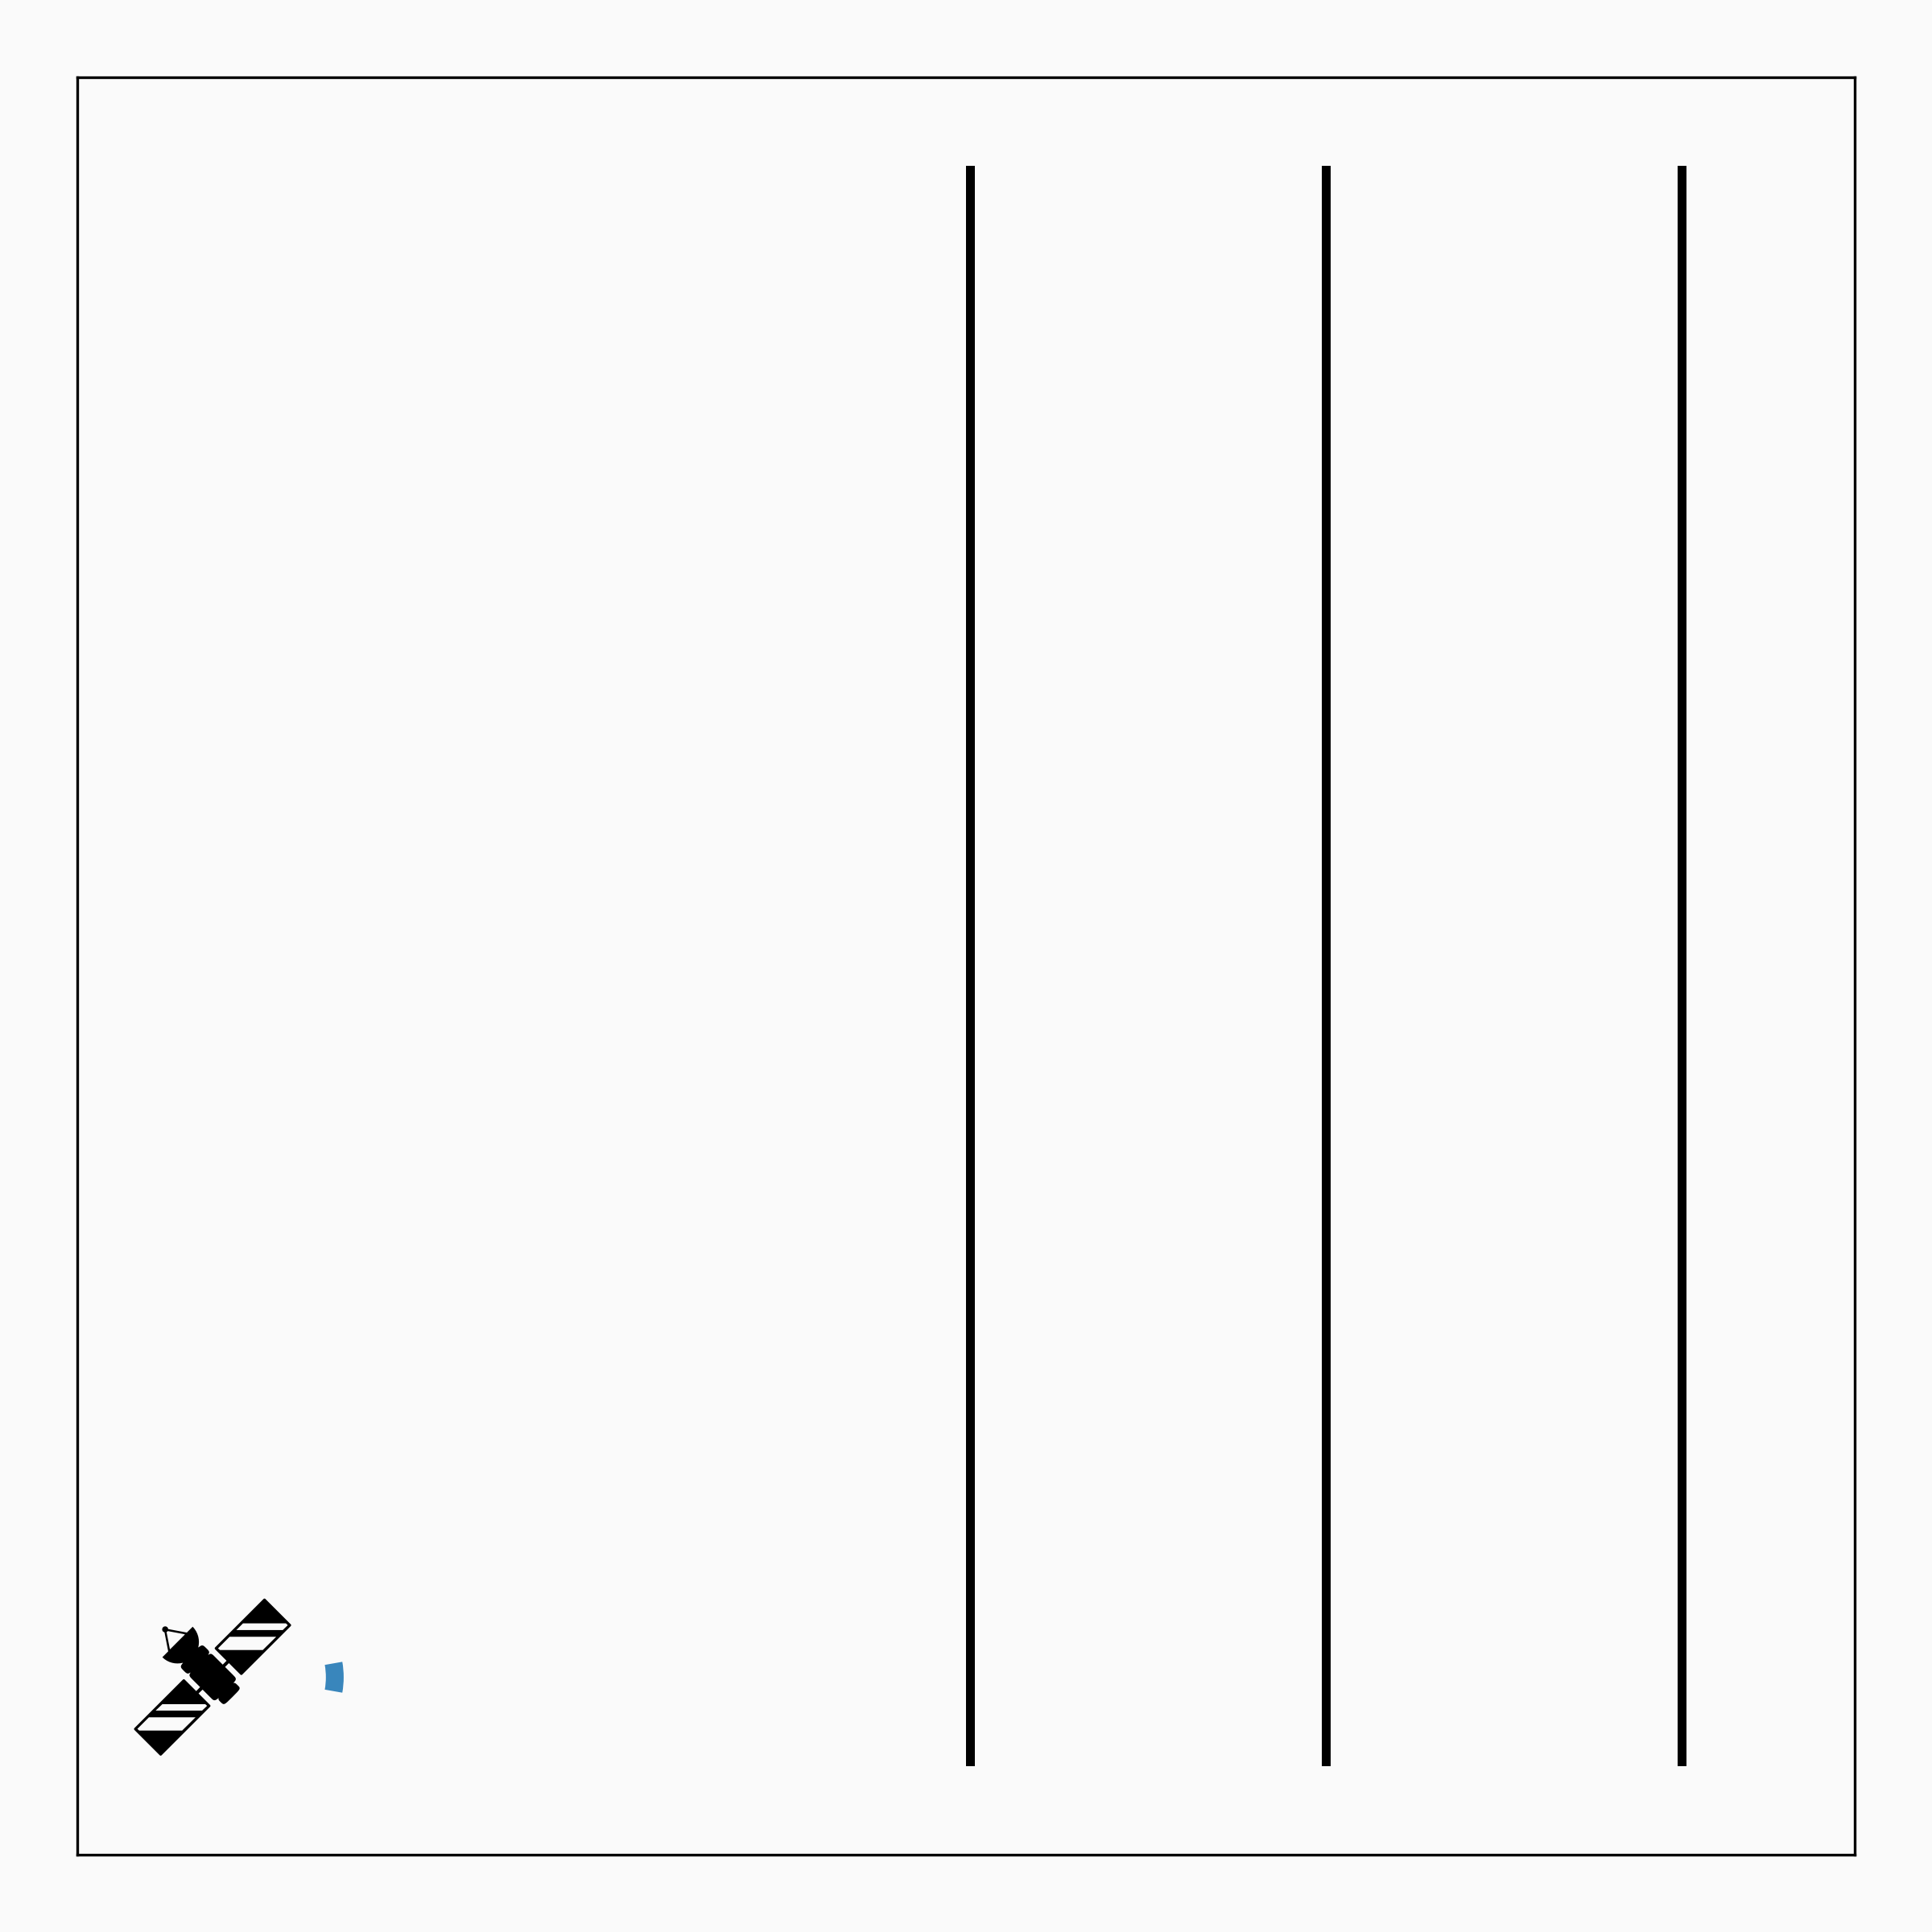
\includegraphics[width=0.95\textwidth]{fig:top.png}}{./figs/fig:top.mp4}
         %\caption{Modo de adquisición STRIPMAP.}
         \label{}
       \end{figure}
    \end{column}
    \begin{column}{0.5\textwidth}  %%<--- here
      \begin{block}{Modo de adquisición TOPSAR}
        \begin{itemize}
          \item El RADAR Va distribuyendo pulsos entre varios swaths y variando el apuntamiento en acimut para iluminar la pisada de manera mas homogénea.
          \item Baja resolución.
          \item Gran cobertura.
          \item Buena distribución de potencia.
        \end{itemize}
      \end{block}
    \end{column}
    \end{columns}
\end{frame}
%--- Next Frame ---%

\begin{frame}{\secname : \subsecname}
\begin{columns}
  \begin{column}{0.5\textwidth}
   \begin{block}{Óptico}
     \begin{itemize}
       \item Rango de trabajo en los micrometros ($0.3\mu$ m a $2.5\mu m$).
       %\item Detecta luz solar reflejada por la tierra.
       \item Afectado por las condiciones atmosféricas.
       %\item Detecta luz incoherente.
       \item Depende de una fuente de iluminación externa.
     \end{itemize}
   \end{block}
  \end{column}
  \begin{column}{0.5\textwidth}  %%<--- here
    \begin{block}{Radar}
      \begin{itemize}
        \item Rango de trabajo en los microondas ($1cm$ m a $100cm$).
        %\item Emite una señal y mide la intesidad del eco.
        \item Independiente de las condiciones atmosféricas.
        %\item Emite y detecta una onda coherente.
        \item Cuenta con su propia fuente de iluminación.
      \end{itemize}
    \end{block}
  \end{column}
  \end{columns}
\end{frame}
%--- Next Frame ---%

\begin{frame}{\secname : \subsecname}
Muchas gracias.
\end{frame}
%--- Next Frame ---%
